\documentclass{article}
\usepackage[T1]{fontenc}
\usepackage[utf8]{inputenc}
\usepackage{amsmath,amssymb,amsfonts}
\usepackage[english,main=russian]{babel}
\usepackage{graphicx}
\graphicspath{{.}}

\begin{document}

\noindent \textbf{1. Пусть есть множество множеств $\{\{1,2,3,4\},\{3,4,5,6\}\}$. Дополните эту систему до:}

\begin{enumerate}

\item(Минимального полукольца) В полукольце должно быть пустое множество - $\emptyset \implies$ множество становится $\{\{1,2,3,4\},\{3,4,5,6\}, \emptyset\}$

В полукольце есть пересечение любых двух элементов $\implies$ множество становится $\{\{1,2,3,4\},\{3,4,5,6\}, \emptyset, \{3,4\}\}$

В полукольце для каждого элемента есть разбиение на элементы из полукольца $\implies$ множество становится 

$\{\{1,2,3,4\},\{3,4,5,6\}, \emptyset, \{3,4\}, \{1,2\}, \{5,6\}\}$
 - это минимальное полукольцо.

\item(Минимального кольца) Любое кольцо - полукольцо. 

Значит $\{\{1,2,3,4\},\{3,4,5,6\}, \emptyset, \{3,4\}, \{1,2\}, \{5,6\}\}$ содержится и в кольце.

Для любых двух элементов из кольца в кольце содержится их симметрическая разность $\implies$ множество становится 

$\{\{1,2,3,4\},\{3,4,5,6\}, \emptyset, \{3,4\}, \{1,2\}, \{5,6\}, \{1,2,5,6\}, \{1,2,3,4,5,6\}\}$


\item(Минимальной алгебры) Полученное нами кольцо

$\{\{1,2,3,4\},\{3,4,5,6\}, \emptyset, \{3,4\}, \{1,2\}, \{5,6\}, \{1,2,5,6\}, \{1,2,3,4,5,6\}\}$ 

является алгеброй.

В данном случае единицей является элемент $\{1,2,3,4,5,6\}$ - он лежит во множестве и пересечение любого элемента с ним дает сам элемент.
\end{enumerate}

\noindent \textbf{2. Доказать, что:}

\begin{enumerate}
\item Пересечение произвольной непустой системы колец является кольцом (возможно, состоящим лишь из пустого множества):

Проверим, что это кольцо, опираясь на определение кольца:

\begin{enumerate}
\item Если во множестве есть элементы $A, B$, то в нем есть $A \cap B$:

От противного: предположим, что в пересечение попали элементы $A, B$, но не $A \cap B$. Т.к. $A, B$ лежат в пересечении, они принадлежат каждому из колец. Но если $A, B$ лежат в кольце, то и $A \cap B$ лежит в кольце. Значит, в каждом кольце есть $A \cap B \implies$ в пересечение колец есть$A \cap B$. Получаем противоречие.

\item  Если во множестве есть элементы $A, B$, то в нем есть $A \triangle B$:

Также как и с предыдущим подпунктом - преположением от противного приходим к выводу, что если $A, B$ лежат в пересечение, то и  $A \triangle B$ лежит в пересчение колец.

\item Отдельным пунктом выделим, что система не пуста:

Т.к. кольцо является и полукольцом, в нем есть $\emptyset$. Значит, и в пересечении колец будет лежать хотя бы $\emptyset$, ведь оно есть в каждом кольце.
\end{enumerate}

\item Пересечение произвольной непустой системы $\sigma$-колец является $\sigma$-кольцом:

$\sigma-$кольцо - это кольцо с счетным объединением. Показано в пункте выше, что пересечение колец - кольцо. Осталось доказать, что полученное кольцо будет $\sigma$-кольцом. 

От противного: пусть в кольце есть такое объединение $\cup_{n \in N}A_n \notin R$. 
Все элементы из пересечения есть в каждом из пересекаемых $\sigma$-колец, а в них 
$\cup_{n \in N}A_n \in R_i (R_i - \text{кольца из пересечения})$. Значит, и $\cup_{n \in N}A_n$ войдет в пересечение. Приходим к противоречию.

\item Пересечение непустой (конечной) системы алгебр с одной и той же единицей является алгеброй:

Алгебра - кольцо с единицей. Уже доказано выше, что пересечение колец - кольцо. Т.к. единица(назовем ее $E$) в каждой алгебре одна и та же, она войдет и в пересечение. И в итоговом кольце $E$ также будет едининцей:

От противного: если $\exists A \text{ из полученного кольца, такой что } A \cap E \neq A$, то этот элемент принадлежит и всем алгебрам. Но в них $A \cap E = A$ - что войдет и в пересечние. Получаем противоречие.

\end{enumerate}

\noindent \textbf{3. Доказать, что следующие множества являются полукольцами с единицей, и указать соответствующие единицы:}

\begin{enumerate}

\item $\{[\alpha;\beta)|a\le\alpha< \beta \le b\} = S$ (включая пустой промежуток): 

Докажем по определению, что это полукольцо:

\begin{enumerate}
\item $\emptyset$ есть в этом множестве по условию - (включая пустой промежуток);

\item Пересечение двух полуинтервалов выглядит следующим образом: 

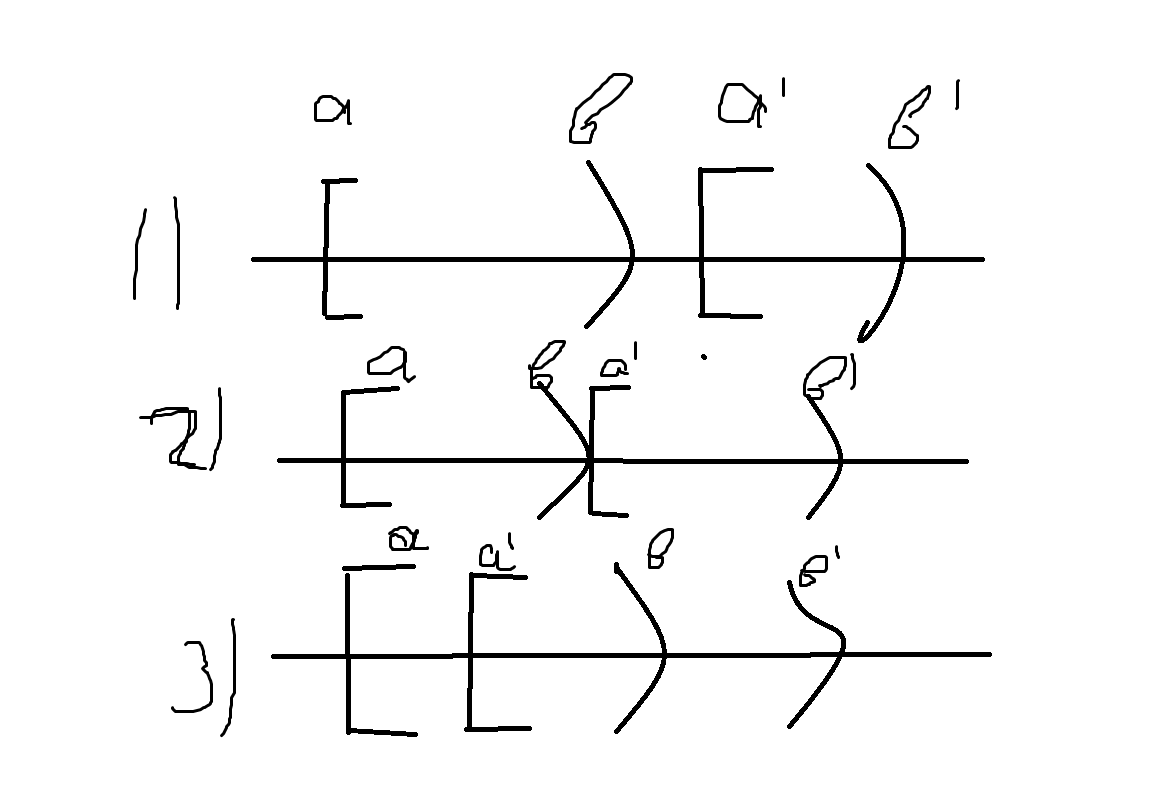
\includegraphics[width=100mm]{Semirings}

Т.е. если у двух полуинтервалов нет ни одной общей точки - их пересчение $\emptyset$; если одна из точек выколота, а другая - нет, то их пересечение также $\emptyset$; иначе в пересечение будет полуинтервал вида: $[c,d) \cap [c',d') = [max(c,c'), min(d,d'))$;

\item Покажем, что для любого полуинтервала найдется разбиение:

От противного предположим, что $\exists [c,d):  a\le c < d \le b$, для которого не существует разбиения. $\exists m: m = \frac{c+d}{2}, m \in [c,d)$

(m $\neq$ d, т.к. это возможно только при $c=d$, что невозможно по условию) $\implies [c,m) \in S \land [m,d) \in S$ - но это разбиение для $[c,d)$, пришли к противоречию.
\end{enumerate}

Единицей для S будет полуинтервал $[a,b)$, т.к. $[a,b) \in S \land \forall [c,d) \in S: [c,d) \cap [a,b) = [c,d)$, т.к. $[c,d) \cap [a,b) = [max(c,a), min(d,b))$ и по условию a - минимальный элемент, b - максимальный.

\item Система всех промежутков, вложенных в отрезок $[a;b]$.

Покажем, что это полукольцо:
\begin{enumerate}
\item Пустое множество принадлежит $[a;b]$ по аналогии с предыдущим пунктом;

\item Какие бы два промежутка из $[a;b]$ мы не выбрали, их пересечение будет лежать в $[a;b]$, потому что это будет либо пустое множество, либо промежуток вида $\{[,(\}max(c,c'), min(d,d')\{],)\}$ - по аналогии с предыдущим пунктом.

\item Разбить промежутки мы можем по аналогии с предыдущим пунктом, только теперь нет ограничения на использование скобок: подойдет как разбиение \{[,(\}c,m), [m,d\{],)\}, так и \{[,(\}c,m], (m,d\{],)\}
\end{enumerate}

Единицей будет являться весь отрезок [a,b].
\end{enumerate}

\noindent \textbf{4. Докажите, что множество всех промежутков с рациональными концами, содержащихся в отрезке $[0;\pi]$, - полукольцо. Почему не кольцо? Есть ли в нем единица?}

Это множество можно выразить так: $S = \{\text{промежуток от $a$ до $b$ }| a,b \in Q \land 0 \le a \le b \le \pi\}$.

По аналогии с предыдущим заданием докажем по определению, что это полукольцо:

\begin{enumerate}
\item $\emptyset$ принадлежит S:

\item Если мы пересечем два промежутка (от с до d, от a до b) с рациональными концами, то в пересечение получится либо пустое множество, либо промежуток, концевые точки которого будут равны max(c,a), min(d,b) - левая и правая соответственно - который также лежит в S по условию.

\item Для разбиения воспользуемся той же техникой, что и в предыдущем задании:
выберем такую точку m на промежутка от а до b, что m = $\frac{a+b}{2} \implies m \in Q$. По условию как \{[,(\}a,m), [m,b\{],)\}, так и \{[,(\}a,m], (m,b\{],)\} лежат в S.
\end{enumerate}

S не будет кольцом, потому нет симметричной разности, например:

$[0,1], [2,3] \in S$, но их симметричная разность $\{[0,1], [2,3]\} \notin S$.

В S нет единицы, т.к. в малой окрестности числа $\pi$ лежит бесконечно много рациональных чисел, поэтому при любом выборе $[0,b]$ - "единицы" - можно будет найти промежуток $[0,b'] : b', b \in Q, b' > b \implies [0,b] \cap [0,b'] = [0,b]$.

\noindent \textbf{5. Пусть A — бесконечное множество, Y — система всех его не более чем счетных подмножеств. Доказать, что Y — $\sigma$-кольцо.}

Докажем по определению:

\begin{enumerate}

\item Пересечение: если два подмножества из Y не более чем счетны, то и их пересечение не более чем счетно $\implies$ пересечение любых двух подмножеств лежит в Y.

\item Симетричная разность: если два подмножества из Y не более чем счетны, то и их симетричная разность не более чем счетна, т.к. каждому элементу из первого подмножества, невходящему в пересечение, мы можем присвоить нечетные номера, каждому элементу из второго, невходящему в пересечение, - четные. Значит, их симметричная разность лежит в Y.

\item Счетное объединение: 
Счетное объединение не более чем счетных множеств будет тоже счетным множеством $\implies$ будет находится в Y. 

Чтобы это доказать, нужно показать, что каждому элементу из объединения можно сопоставить какое-либо $n \in N$. 

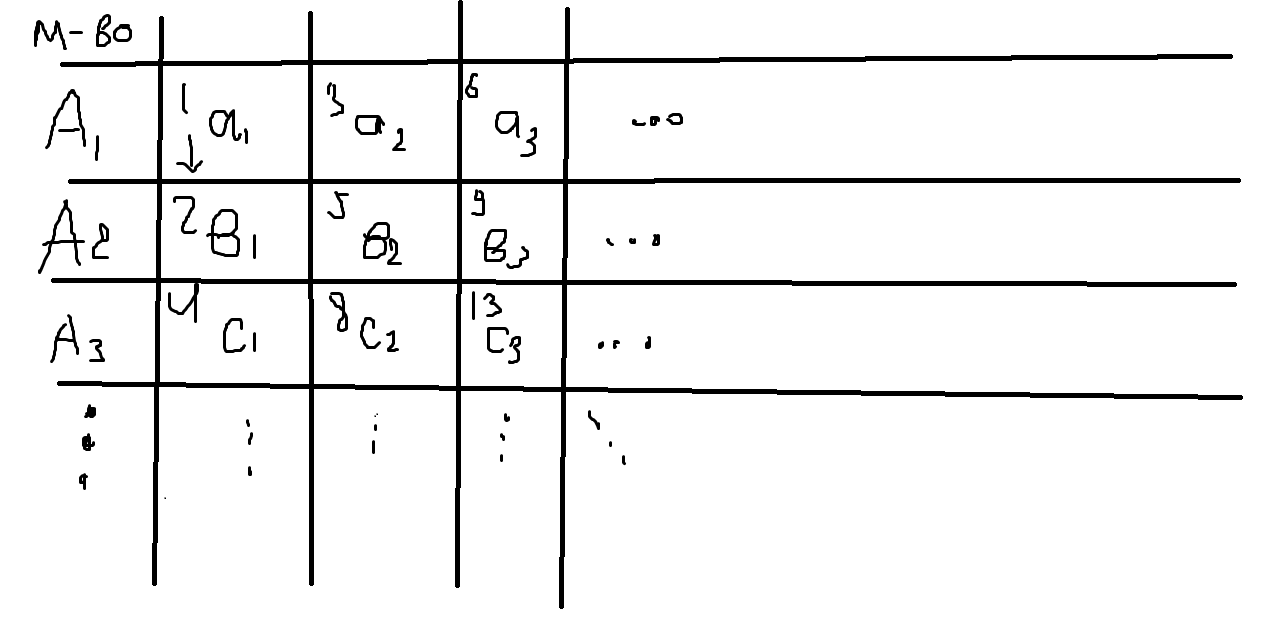
\includegraphics[width=100mm]{Table}

Элементы каждого из объединяемых множеств можно записать в строку и пронумеровать их по побочным диагоналям получившейся таблицы - точно также, как доказывается счетность рациональных чисел. 

\end{enumerate}

\end{document}